\begin{figure*}[h]
  \begin{center}
    \begin{tabular}{c}
      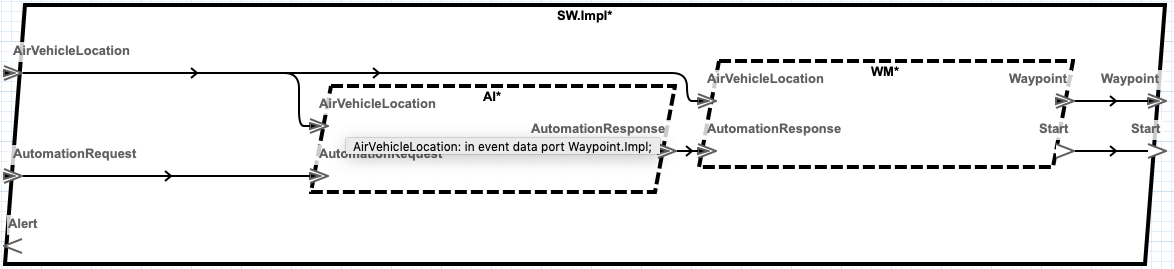
\includegraphics[scale=0.4]{example.png}
    \end{tabular}
  \end{center}
\caption{Initial design for an automated UAV route planning system.}
\label{fig:example}
\end{figure*}

\begin{figure}
  \begin{center}
    \begin{tabular}{c}
      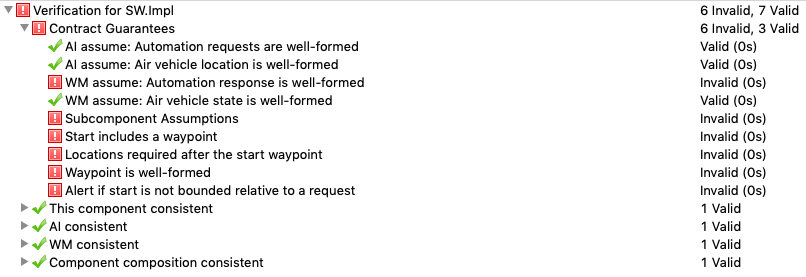
\includegraphics[scale=0.4]{example-certificate.png} \\
    \end{tabular}
  \end{center}
\caption{AGREE failure certificate for initial design.}
\label{fig:example-certificate}
\end{figure}

\figref{fig:example} is an AADL architectural model of a software system (SW) for route planning and automated control of a UAV.
It is loosely based on one of the case studies in Section~\ref{sec:case-study}.
The source for the entire model is found at \cite{repo}.

The system receives an automation request that is forwarded to a third-party route planner (AI).
The route planner decides the flight path of the UAV based on its current position and the requested task.
The waypoint manager (WM) receives the mission command as a set of waypoints from the planner and starts the UAV flying the mission, issuing waypoints to the UAV flight controller as the UAV location changes.
The waypoint manager is a repurposed legacy component that cannot be modified.

The expected behavior of the SW system, and the components in its implementation, are specified (i.e., modeled) with AGREE contract specifications.
The contracts constrain input with assumptions and state properties of output with guarantees.
AGREE performs model checking on this assume-guarantee system to hierarchically prove that the composite system obeys all contract obligations under all possible finite input streams. 
The AGREE contracts for the system and its implementing components are discussed in greater detail in \secref{sec:agree}.

The initial contract for the system in \figref{fig:example}, and its implementing components, assume and guarantee the absence of any malicious, or underspecified, component behavior.
The system assumes that all inputs are \emph{well-formed} and there is never more than one automation request pending at a time.
The meaning of well-formed is given by predicates for each data type.
For example, a waypoint is well-formed if it falls within bounds for latitude, longitude, and altitude.
The system guarantees that a start includes a waypoint, a start is within one cycle of an automation request and if not, then it persistently alerts, new waypoints coincide with air vehicle location updates, and all output are well-formed.

The components assume their inputs are well-formed, and they guarantee their outputs are well-formed.
The AI further guarantees it only responds to automation requests and always in the same cycle.
The legacy WM further guarantees a start from a response and always in the same cycle, start always comes with a waypoint, and further waypoints coincide with air vehicle location updates.
This system implementation passes AGREE verification meaning that the contract composition of the components with the system satisfies all component input assumptions and system output guarantees.

A cyber-vulnerability analysis identifies the potential of a supply chain attack through the AI route planner provided by the third-party vendor without source code.
The component is marked as \emph{untrusted}, and its contract is modified by removing all guarantees on its outputs to reflect its untrusted status.
The AI output is now unconstrained in the assume-guarantee reasoning of AGREE and is able to generate any value on its output stream at anytime.
AGREE must consider all possible output streams from the AI in proving the correctness of the component implementation of the automated UAV route planning system.

The output from AGREE with the AI specification is shown in \figref{fig:example-certificate}.
The red exclamation points designate component assumptions or system output guarantees that do not hold, and each failure comes with a corresponding counter-example.
The results are not unexpected given the AI route planner's unconstrained behavior.

For example, the first violation is that the automation response from the AI to the WM is no longer guaranteed to be well-formed.
The consequence of that failing input assumption is that the WM outputs are no longer guaranteed; they are effectively unconstrained.
These missing output guarantees from the WM lead to the rest of the failures in \figref{fig:example-certificate} because the WM provides the system level outputs.

\begin{figure*}
  \begin{center}
    \begin{tabular}{c}
      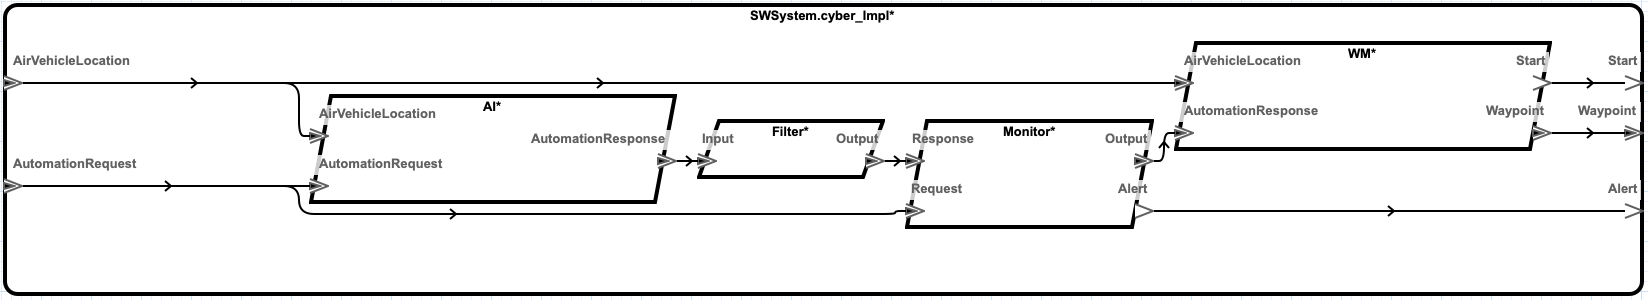
\includegraphics[scale=0.3]{hardened.png}
    \end{tabular}
  \end{center}
  \caption{Cyber-hardened design for an automated UAV route planning system}
  \label{fig:hardened}
\end{figure*}

\begin{figure}
  \begin{center}
    \begin{tabular}{c}
      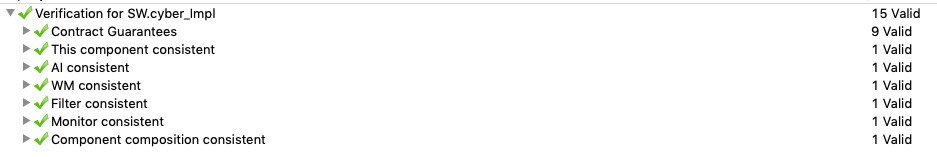
\includegraphics[scale=0.4]{hardened-certificate.png}
    \end{tabular}
  \end{center}
  \caption{AGREE verification certificate for cyber-hardened design.}
  \label{fig:hardened-certificate}
\end{figure}

The system implementation is cyber-hardened using BriefCASE, which automatically transforms the model by inserting high-assurance components in the form of a filter and a monitor as shown in \figref{fig:hardened}.
A filter enforces an invariant over each datum in the data stream by not forwarding input to its output if that input violates the filter invariant.
The auto-generated AGREE specification states that only well-formed inputs are passed to the output.
The system developer must provide this filtering policy, but it is usually based on the existing assumptions made by downstream components that consume the filter output. 

A monitor captures a relation on input data over time and is thus able to reason about temporal properties of that input.
A monitor raises an alert if the specified temporal properties are ever violated.
The AGREE specification for the monitor in our example states that an automation response can only be generated in conjunction with an automation request; and further, that response must come with the request or in the next step after the request.
As with the filter, the system designer provides the policy, and that policy is based on the existing AGREE specification in the SW system.

The AGREE analysis of the cyber-hardened implementation with the auto-generated high-assurance components is shown in \figref{fig:hardened}.
Here AGREE provides a proof certificate that the high-assurance components guarantee the correct behavior of the SW implementation in the presence of the untrusted AI route planner.

The high-assurance components are automatically synthesized by SPLAT from the AGREE specifications to equivalent models in the CakeML language.
CakeML itself provides a complete verified compilation to binaries for several different platforms meaning that the resulting binaries exactly preserve the meaning of the original CakeML code \cite{cakeml}. 

A similar proof is given for the synthesis of the contract model for a high-assurance component to CakeML.
A high-assurance component contract has a precise meaning in terms of data streams, and the synthesis exactly preserves that meaning in the generated code.
In other words, for any set of input streams that meet the component's contract assumptions, the output streams produced from the synthesized CakeML code exactly match those defined by the high-assurance component's contract. 

Preserving the input to output relationship of streams between the two models lifts the contract verification results to the deployed system.
If the contract model verification succeeds, then the meaning of those results hold for the deployed system, given that all other components implement their contracts, an appropriate schedule exists that follows the dependent data-flow, and the communication fabric works as expected.
